\documentclass{ximera}
% \usepackage{tikz}
% \usepackage{pgfplots}
% ../preamble.tex
% \addPrintStyle{..}

\begin{document}
    \xmtitle{TikZ: height issue}{}

    START
%     \begin{image}
%         {\def\length{sqrt(1+(x+y)^2)}
%         \begin{tikzpicture}
%           \begin{axis}[
%               xmin=-3, xmax=3,ymin=-3,ymax=3,domain=-3:3,view={0}{90},
%               axis lines =center, xlabel=$x$, ylabel=$y$,
%               every axis y label/.style={at=(current axis.above origin),anchor=south},
%               every axis x label/.style={at=(current axis.right of origin),anchor=west},
%               axis on top,
%             ]
%             \addplot3 [blue, quiver={u={1/\length}, v={(x+y)/(\length)},scale arrows=.2},samples=20] {0};
%             \addplot[blue,very thick]{e^x-x-1};
%             \addplot[blue,very thick]{.2*e^x-x-1};
%             \addplot[blue,very thick]{-e^x-x-1};
%             \addplot[blue,very thick]{-.2*e^x-x-1};
%             \addplot[blue,very thick]{-3*e^x-x-1};
%             \addplot[blue,very thick]{2*e^x-x-1};
%             \addplot[blue,very thick]{-x-1};
%         \end{axis}
%         \end{tikzpicture}}
%     \end{image}
% END
%\begin{image}
    {\def\length{sqrt(1+(x+y)^2)}
    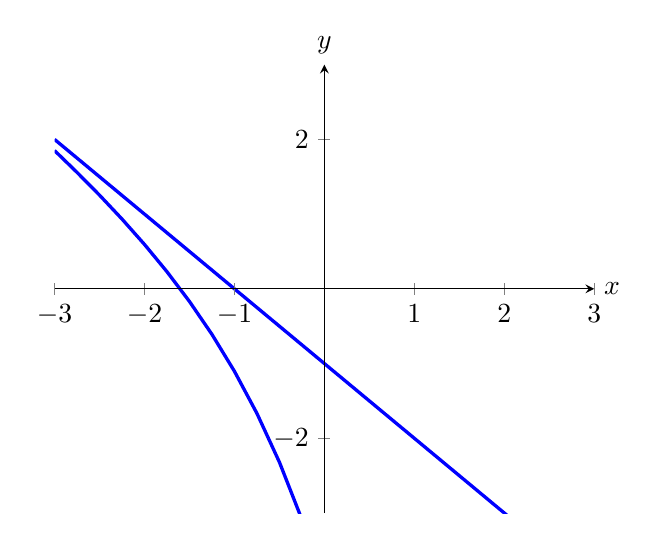
\begin{tikzpicture}
      \begin{axis}[
          xmin=-3, xmax=3,ymin=-3,ymax=3,domain=-3:3,
          %view={0}{90},
          axis lines =center, xlabel=$x$, ylabel=$y$,
          every axis y label/.style={at=(current axis.above origin),anchor=south},
          every axis x label/.style={at=(current axis.right of origin),anchor=west},
          axis on top,
        ]
    %    \addplot3 [blue, quiver={u={1/\length}, v={(x+y)/(\length)},scale arrows=.2},samples=20] {0};
        % \addplot[blue,very thick]{e^x-x-1};
        % \addplot[blue,very thick]{.2*e^x-x-1};
        % \addplot[blue,very thick]{-e^x-x-1};
        % \addplot[blue,very thick]{-.2*e^x-x-1};
        \addplot[blue,very thick]{-3*e^x-x-1};
        % \addplot[blue,very thick]{2*e^x-x-1};
        \addplot[blue,very thick]{-x-1};
    \end{axis}
    \end{tikzpicture}}
%\end{image}
END2

\end{document}